% vim:autoindent:set textwidth=78:

\section{Trabajar con proyecciones}\label{label_projections}
\index{projections!working with}

QGIS soporta la proyección al vuelo de capas vectoriales. Esta función permite visualizar capas con diferente sistema de coordenadas y superponerlas de forma adecuada.

\subsection{Descripción del soporte para proyecciones}\label{label_projoverview}

QGIS tiene soporte para aproximadamente 2.700 proyecciones conocidas. Las proyecciones se guardan en una base de datos de Sqlite que se instala con QGIS.
%Appendix \ref{app:datamodel}  contains information about the database and the
% schema. 
Normalmente no se necesita manipular la base de datos directamente. De hecho, hacerlo puede ocasionar que falle el soporte de proyecciones. Las proyecciones personalizadas se guardan en una base de datos del usuario. Ver la sección \ref{sec:customprojections} para información sobre la gestión de sus proyecciones personalizadas.

Las proyecciones disponibles en QGIS están basadas en aquellas definidas por EPSG\index{EPSG} y están ampliamente resumidas de la tabla de referencias\_espaciales de PostGIS\index{PostGIS} versión 1.x. Note que los identificadores usados en QGIS no se corresponden con los de EPSG o PostGIS. Los identificadores EPSG y PostGIS están presentes en la base de datos y se pueden usar para especificar una proyección en QGIS.

Para usar una proyección al vuelo, sus datos deben contener información sobre su sistema de coordenadas. Para capas PostGIS QGIS usa el identificador de referencia espacial que se especificó cuando se creó la capa. Para datos soportados por OGR, QGIS se base en la presencia de un medio específico del formato para definir el sistema de coordenadas. En el caso archivos shape, esto significa un archivo que contenga la especificación WTK (Well Known Text) \index{WKT} del sistema de coordenadas. El archivo de proyección tiene el mismo nombre base que el archivo shape y una extensión prj. Por ejemplo, un archivo shape que se llame lagos.shp tendrá un archivo de proyección correspondiente llamado lagos.prj.

%\section{Requirements}
%QGIS uses the Proj4 to provide proyection support. 

\subsection{Comenzar}\label{label_projstart}

Al inicio, QGIS no tiene la proyección al vuelo habilitada. Para usar la proyección al vuelo, debe abrir el diálogo \textit{Propiedades del proyecto}, seleccionar una proyección para el mapa y activar la proyección al vuelo. Hay dos formas de abrir el diálogo \textit{Propiedades del proyecto}:

\begin{enumerate}
\item Seleccionar \textit{Propiedades del proyecto} del menú \textit{Configuración}.
\item Hacer clic en el icono del proyector en la esquina inferior derecha de la barra de estado.
\end{enumerate}

\begin{Tip}
 \caption{\textsc{Diálogo Propiedades del proyecto}}
\qgistip{
Si abre el diálogo \textit{Propiedades del proyecto} desde el menú \textit{Configuración}, debe hacer clic en la pestaña \textit{Proyección} para ver la configuración de la proyección. Abriendo el diálogo desde el icono del proyector llevará directamente la pestaña \textit{Proyección} al frente.
}
\end{Tip}

El diálogo Proyección contiene cuatro componentes importantes tal como se numeran en la Figura \ref{fig:projections} y se describe a continuación.

\begin{figure}[ht]
   \begin{center}
   \caption{Diálogo Proyección (GNU/Linux)}\label{fig:projections}\smallskip
   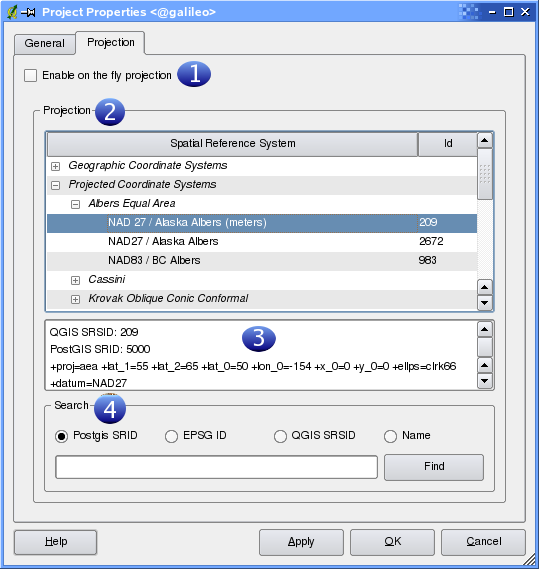
\includegraphics[clip=true, width=14cm]{projectiondialog08}
\end{center}  
\end{figure}

\begin{enumerate}
\item \textbf{Activar proyección al vuelo}\index{projections!enabling} - esta casilla de verificación se usa para activar o desactivar la proyección al vuelo. Cuando no está marcada, no se proyecta nada y cada capa se dibuja usando las coordenadas leídas de la fuente de datos. Cuando está marcada, las coordenadas de cada capa se proyectan al sistema de coordenadas de la vista del mapa.
\item \textbf{Proyecciones} - esta es una lista de todas las proyecciones soportadas por QGIS, incluyendo sistemas de coordenadas geográficas, proyectadas y personalizadas. Para usar un sistema de coordenadas, selecciónelo de la lista expandiendo la rama adecuada y seleccionando la proyección. La proyección activa está preseleccionada.
\item \textbf{Texto Proj4} - esta es la cadena de la proyección usada por el motor de proyección Proj4. Este texto es de sólo lectura y se proporciona con finalidad informativa.
\item \textbf{Buscar} - si conoce el identificador PostGIS, EPSG o QGIS SRSID o el nombre de una proyección, puede usar la función de búsqueda para encontrarlo. Introduzca el identificador y pulse \textit{Encontrar}.
\end{enumerate}

\subsubsection{Especificar una proyección}
\index{projections!specifying}
\label{sec:proyección-specifying}

QGIS establece automáticalmente la proyección del mapa al sistema de coordenadas de la primera capa cargada. Una forma de especificar la proyección del mapa es cargar primero una capa con la proyección que quiera para todo el mapa. A continuación abra el diálogo \textit{Propiedades del proyecto} y marque la casilla \textit{Activar
proyección al vuelo}. Ahora puede cerrar el diálogo \textit{Propiedades del proyecto} y añadir capas adicionales al mapa. 

Si ya ha añadido capas y quiere activar la proyección al vuelo, abra el diálogo \textit{Propiedades del proyecto} y busque el sistema de coordenadas proyectadas o geográficas que quiera usar en la lista de proyecciones. Alternativamente puede usar la función de búsqueda como se describe en la sección anterior.

\subsection{Proyecciones personalizadas}\label{sec:customprojections}
\index{projections!custom}

Si QGIS no tiene la proyección que necesita, puede definir una proyección personalizada. Para definir una proyección, seleccione \textit{Proyección personalizada} del menú \textit{Configuración}. Las proyecciones personalizadas se guardan en su base de datos de usuario de QGIS. Además de sus proyecciones, esta base de datos contiene sus marcadores espaciales y otros datos de usuario. 

\begin{figure}[ht]
   \begin{center}
   \caption{Diálogo Proyección personalizada (OS X)}\label{fig:customprojections}\smallskip
   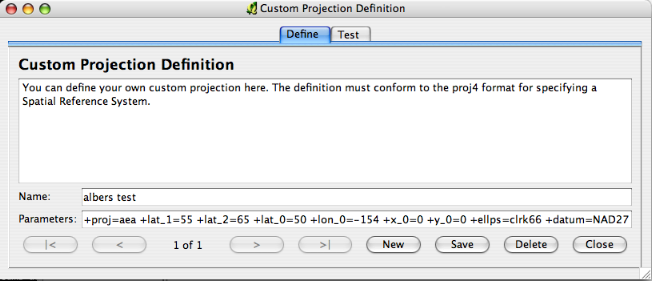
\includegraphics[clip=true, width=14cm]{customprojection}
\end{center}  
\end{figure}

En la versión \CURRENT de QGIS, definir una proyección personalizada requiere un buen conocimiento de la biblioteca de proyecciones Proj.4. Para empezar, consulte el documento Cartographic Projection Procedures for the UNIX Environment - A User's Manual
by Gerald I. Evenden, U.S. Geological Survey Open-File Report 90-284, 1990
(disponible en \url{ftp://ftp.remotesensing.org/proj/OF90-284.pdf}).
Este manual describe el uso del comando \textit{proj} y utilidades relacionadas de línea de comandos. Los parámetros cartográficos usados con \textit{proj} y descritos en el manual son los mismos que usa QGIS. 

El diálogo \textit{Proyecciones personalizadas} sólo requiere dos parámetros para definir una proyección de usuario: 
\begin{enumerate}
\item un nombre descriptivo y
\item los parámetros cartográficos. 
\end{enumerate}
Para crear una nueva proyección, pulse el botón \textit{Nueva} e introduzca un nombre descriptivo y los parámetros de la proyección. La figura \ref{fig:customprojections} muestra el diálogo con una proyección de ejemplo. Los parámetros mostrados fueron introducidos en base al conocimiento de la proyección y la información encontrada en OF90-284.

Puede probar los parámetros de su proyección para ver si dan buen resultado haciendo clic en la pestaña \textit{Probar} y pegando los parámetros de su proyección en el campo \textit{Parámetros}. Introduzca a continuación valores conocidos de latitud y longitud WGS 84 en los campos Norte y Este respectivamente. Pulse en \textit{Calcular} y compare los resultados con los valores conocidos en su sistema de coordenadas proyectadas. 
